% ===========================================================================
%  TikuOS — TikuKits DS: Ring Buffer for Embedded Systems
%  Beamer Presentation
% ===========================================================================
\documentclass[aspectratio=169, 10pt]{beamer}

% ---- Theme ----------------------------------------------------------------
\usetheme{Madrid}
\usecolortheme{whale}
\setbeamertemplate{navigation symbols}{}
\setbeamertemplate{footline}{%
  \leavevmode\hbox{%
    \begin{beamercolorbox}[wd=.33\paperwidth,ht=2.5ex,dp=1ex,center]{author in head/foot}%
      \usebeamerfont{author in head/foot}\insertshortauthor
    \end{beamercolorbox}%
    \begin{beamercolorbox}[wd=.34\paperwidth,ht=2.5ex,dp=1ex,center]{title in head/foot}%
      \usebeamerfont{title in head/foot}\insertshorttitle
    \end{beamercolorbox}%
    \begin{beamercolorbox}[wd=.33\paperwidth,ht=2.5ex,dp=1ex,right]{date in head/foot}%
      \usebeamerfont{date in head/foot}\insertshortdate{}\hspace*{2em}%
      \insertframenumber{}/\inserttotalframenumber\hspace*{2ex}
    \end{beamercolorbox}}%
  \vskip0pt%
}

% ---- Packages -------------------------------------------------------------
\usepackage{listings}
\usepackage{graphicx}
\usepackage{hyperref}
\usepackage{booktabs}
\usepackage{multirow}
\usepackage{tikz}
\usetikzlibrary{arrows.meta, positioning, shapes.geometric, calc,
                decorations.pathreplacing, fit}
\usepackage{amsmath}

% ---- Code listing style ---------------------------------------------------
\lstset{
  basicstyle=\ttfamily\scriptsize,
  keywordstyle=\color{blue}\bfseries,
  commentstyle=\color{gray},
  stringstyle=\color{red!70!black},
  showstringspaces=false,
  breaklines=true,
  frame=single,
  rulecolor=\color{black!30},
  backgroundcolor=\color{blue!3},
  tabsize=4,
}
\lstdefinestyle{cstyle}{
  language=C,
  morekeywords={uint8_t,uint16_t,uint32_t,int32_t,int16_t,
                tiku_kits_ds_elem_t,
                TIKU_KITS_DS_OK,TIKU_KITS_DS_ERR_NULL,
                TIKU_KITS_DS_ERR_FULL,TIKU_KITS_DS_ERR_EMPTY,
                TIKU_KITS_DS_ERR_PARAM,TIKU_KITS_DS_ERR_NOTFOUND,
                TIKU_KITS_DS_ERR_BOUNDS,
                TIKU_KITS_DS_RINGBUF_MAX_SIZE,
                NULL},
}

% ---- Metadata -------------------------------------------------------------
\title[TikuKits DS]{TikuKits DS: Ring Buffer for Embedded Systems}
\subtitle{Simple. Ubiquitous. Intelligence, Everywhere.}
\author[Ambuj Varshney]{Ambuj Varshney \\ \texttt{ambuj@tiku-os.org}}
\date{\today}

% ===========================================================================
\begin{document}

% ---------------------------------------------------------------------------
\begin{frame}
\titlepage
\end{frame}

% ---------------------------------------------------------------------------
\begin{frame}{Outline}
\tableofcontents
\end{frame}

% ===========================================================================
\section{Motivation}
% ===========================================================================

\begin{frame}{Why a Ring Buffer on MCUs?}
\begin{columns}[T]
\begin{column}{0.48\textwidth}
\begin{block}{Embedded Use Cases}
\begin{itemize}
  \item \textbf{UART receive buffer} --- ISR pushes bytes, main loop pops
  \item \textbf{Last-N sensor samples} --- keep recent history in fixed memory
  \item \textbf{Event queue} --- decouple interrupt producers from consumers
  \item \textbf{Audio/signal streaming} --- bounded buffering between stages
\end{itemize}
\end{block}

\begin{block}{Constraints}
\begin{itemize}
  \item No heap allocation
  \item Fixed, bounded memory usage
  \item $O(1)$ push and pop --- hard real-time safe
  \item ISR-safe producer / main-loop consumer
\end{itemize}
\end{block}
\end{column}

\begin{column}{0.48\textwidth}
\begin{center}
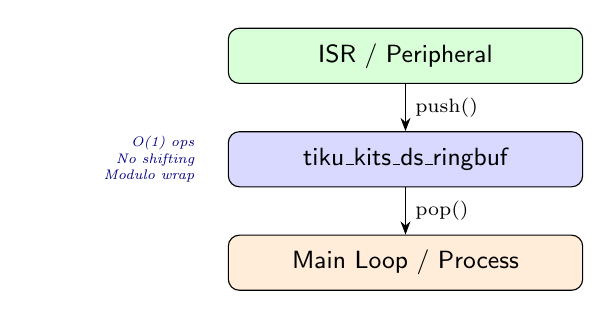
\begin{tikzpicture}[
    >=Stealth, node distance=0.5cm
  ]
  \node[draw, rounded corners, minimum height=0.7cm,
        text centered, font=\small\sffamily, fill=green!15,
        minimum width=4.5cm] (isr) {ISR / Peripheral};
  \node[draw, rounded corners, minimum height=0.7cm,
        text centered, font=\small\sffamily, fill=blue!15,
        minimum width=4.5cm, below=0.6cm of isr] (rb)
    {tiku\_kits\_ds\_ringbuf};
  \node[draw, rounded corners, minimum height=0.7cm,
        text centered, font=\small\sffamily, fill=orange!15,
        minimum width=4.5cm, below=0.6cm of rb] (main)
    {Main Loop / Process};
  \draw[->] (isr) -- node[right, font=\scriptsize] {push()} (rb);
  \draw[->] (rb) -- node[right, font=\scriptsize] {pop()} (main);

  \node[left=0.3cm of rb, font=\tiny\itshape, text=blue!50!black,
        text width=2cm, align=right] {O(1) ops\\No shifting\\Modulo wrap};
\end{tikzpicture}
\end{center}

\vspace{0.5em}
\begin{alertblock}{Design Goal}
Provide a fixed-size circular buffer with $O(1)$ push/pop,
\textbf{no wasted slots}, and a separate count field to distinguish
full from empty.
\end{alertblock}
\end{column}
\end{columns}
\end{frame}

% ===========================================================================
\section{Data Structure}
% ===========================================================================

\begin{frame}[fragile]{The \texttt{tiku\_kits\_ds\_ringbuf} Structure}
\begin{columns}[T]
\begin{column}{0.48\textwidth}
\begin{lstlisting}[style=cstyle,
  title={ds/ringbuf/tiku\_kits\_ds\_ringbuf.h}]
#ifndef TIKU_KITS_DS_RINGBUF_MAX_SIZE
#define TIKU_KITS_DS_RINGBUF_MAX_SIZE 32
#endif

struct tiku_kits_ds_ringbuf {
    tiku_kits_ds_elem_t
        data[TIKU_KITS_DS_RINGBUF_MAX_SIZE];
    uint16_t head;      /* read position  */
    uint16_t tail;      /* write position */
    uint16_t count;     /* valid elements */
    uint16_t capacity;  /* user limit     */
};
\end{lstlisting}

\vspace{0.3em}
\textbf{Memory footprint:}\\
$32 \times 4 + 4 \times 2 = 136$ bytes (default).\\
All statically allocated --- no heap.
\end{column}

\begin{column}{0.48\textwidth}
\textbf{Circular buffer layout:}
\begin{center}
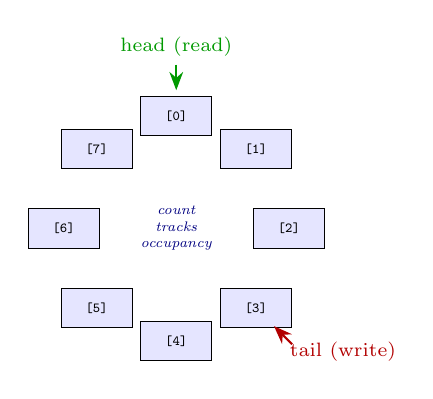
\begin{tikzpicture}[>=Stealth, scale=0.65]
  % Draw circular slots
  \foreach \i in {0,...,7} {
    \pgfmathsetmacro{\angle}{90 - \i * 45}
    \node[draw, minimum width=0.9cm, minimum height=0.5cm,
          fill=blue!10, font=\tiny\ttfamily,
          rotate=0] at (\angle:2.2cm) {[\i]};
  }

  % Head arrow
  \draw[->, thick, green!60!black] (90:3.2cm) -- (90:2.7cm)
    node[above=0.3cm, font=\scriptsize] {head (read)};

  % Tail arrow
  \draw[->, thick, red!70!black] (-45:3.2cm) -- (-45:2.7cm)
    node[below right=0.1cm, font=\scriptsize] {tail (write)};

  % Center label
  \node[font=\tiny\itshape, text=blue!50!black, align=center] at (0,0) {count\\tracks\\occupancy};
\end{tikzpicture}
\end{center}

\vspace{0.5em}
\begin{block}{Full vs. Empty}
\begin{itemize}
  \item \texttt{count == 0}: empty
  \item \texttt{count == capacity}: full
  \item No wasted slot --- all capacity usable
\end{itemize}
\end{block}
\end{column}
\end{columns}
\end{frame}

% ===========================================================================
\section{API Reference}
% ===========================================================================

\begin{frame}[fragile]{Complete API}
\begin{table}
\centering
\small
\begin{tabular}{@{}lp{8cm}@{}}
\toprule
\textbf{Function} & \textbf{Description} \\
\midrule
\texttt{\_ringbuf\_init(rb, cap)}
  & Initialize with capacity $1 \ldots$ \texttt{MAX\_SIZE}; zeros data \\
\texttt{\_ringbuf\_push(rb, val)}
  & Write at tail, advance tail via modulo; returns \texttt{ERR\_FULL} \\
\texttt{\_ringbuf\_pop(rb, \&val)}
  & Read from head, advance head via modulo; returns \texttt{ERR\_EMPTY} \\
\texttt{\_ringbuf\_peek(rb, \&val)}
  & Read head element without removing it \\
\midrule
\texttt{\_ringbuf\_clear(rb)}
  & Reset head, tail, count to 0 \\
\texttt{\_ringbuf\_count(rb)}
  & Return current number of elements \\
\texttt{\_ringbuf\_full(rb)}
  & Return 1 if count $\geq$ capacity \\
\texttt{\_ringbuf\_empty(rb)}
  & Return 1 if count $=$ 0 \\
\bottomrule
\end{tabular}
\end{table}

\vspace{0.3em}
{\scriptsize All functions are prefixed with \texttt{tiku\_kits\_ds}.
Every function validates pointer arguments and returns \texttt{ERR\_NULL} on failure.}

\begin{alertblock}{No Silent Overwrite}
When the buffer is full, \texttt{push()} returns \texttt{ERR\_FULL} --- it
does \emph{not} silently overwrite the oldest element. The caller decides
the policy (drop, pop-then-push, etc.).
\end{alertblock}
\end{frame}

% ===========================================================================
\section{How It Works}
% ===========================================================================

\begin{frame}[fragile]{Modulo Wrap Arithmetic}
\begin{columns}[T]
\begin{column}{0.48\textwidth}
\begin{lstlisting}[style=cstyle,
  title={push --- write at tail, wrap}]
int tiku_kits_ds_ringbuf_push(
    struct tiku_kits_ds_ringbuf *rb,
    tiku_kits_ds_elem_t value)
{
    if (rb == NULL)
        return TIKU_KITS_DS_ERR_NULL;
    if (rb->count >= rb->capacity)
        return TIKU_KITS_DS_ERR_FULL;

    rb->data[rb->tail] = value;
    rb->tail = (rb->tail + 1)
               % rb->capacity;
    rb->count++;
    return TIKU_KITS_DS_OK;
}
\end{lstlisting}
\end{column}

\begin{column}{0.48\textwidth}
\begin{lstlisting}[style=cstyle,
  title={pop --- read from head, wrap}]
int tiku_kits_ds_ringbuf_pop(
    struct tiku_kits_ds_ringbuf *rb,
    tiku_kits_ds_elem_t *value)
{
    if (rb == NULL || value == NULL)
        return TIKU_KITS_DS_ERR_NULL;
    if (rb->count == 0)
        return TIKU_KITS_DS_ERR_EMPTY;

    *value = rb->data[rb->head];
    rb->head = (rb->head + 1)
               % rb->capacity;
    rb->count--;
    return TIKU_KITS_DS_OK;
}
\end{lstlisting}
\end{column}
\end{columns}

\vspace{0.3em}
\begin{block}{Key Insight: Modulo Wrapping}
\[
  \texttt{tail} = (\texttt{tail} + 1) \bmod \texttt{capacity}
\]
When the index reaches the end of the array it wraps back to 0.
No element shifting, no memmove --- constant-time $O(1)$ for both push and pop.
\end{block}
\end{frame}

% ===========================================================================
\section{Code Examples}
% ===========================================================================

\begin{frame}[fragile]{Example 1: Basic Push, Pop, and Peek}
\begin{lstlisting}[style=cstyle,
  title={Basic ring buffer usage}]
#include "tikukits/ds/ringbuf/tiku_kits_ds_ringbuf.h"

struct tiku_kits_ds_ringbuf rb;
tiku_kits_ds_elem_t val;

/* Initialize with capacity 4 */
tiku_kits_ds_ringbuf_init(&rb, 4);

/* Push three values */
tiku_kits_ds_ringbuf_push(&rb, 10);
tiku_kits_ds_ringbuf_push(&rb, 20);
tiku_kits_ds_ringbuf_push(&rb, 30);
/* count == 3, head == 0, tail == 3 */

/* Peek reads head without removing */
tiku_kits_ds_ringbuf_peek(&rb, &val);     /* val == 10 */

/* Pop returns oldest first (FIFO) */
tiku_kits_ds_ringbuf_pop(&rb, &val);      /* val == 10 */
tiku_kits_ds_ringbuf_pop(&rb, &val);      /* val == 20 */
/* count == 1, head == 2 */

/* Check state */
int is_empty = tiku_kits_ds_ringbuf_empty(&rb);   /* 0 */
uint16_t n   = tiku_kits_ds_ringbuf_count(&rb);   /* 1 */
\end{lstlisting}
\end{frame}

% ---------------------------------------------------------------------------
\begin{frame}[fragile]{Example 2: Wraparound in Action}
\begin{columns}[T]
\begin{column}{0.48\textwidth}
\begin{lstlisting}[style=cstyle,
  title={Fill, drain, refill --- tail wraps}]
struct tiku_kits_ds_ringbuf rb;
tiku_kits_ds_elem_t val;

tiku_kits_ds_ringbuf_init(&rb, 4);

/* Fill: [10, 20, 30, 40] */
tiku_kits_ds_ringbuf_push(&rb, 10);
tiku_kits_ds_ringbuf_push(&rb, 20);
tiku_kits_ds_ringbuf_push(&rb, 30);
tiku_kits_ds_ringbuf_push(&rb, 40);
/* head=0, tail=0 (wrapped), count=4 */

/* Pop two: head advances to 2 */
tiku_kits_ds_ringbuf_pop(&rb, &val); /* 10 */
tiku_kits_ds_ringbuf_pop(&rb, &val); /* 20 */

/* Push two more: tail wraps to 2 */
tiku_kits_ds_ringbuf_push(&rb, 50);
tiku_kits_ds_ringbuf_push(&rb, 60);
/* full again: count=4 */

/* Pop all: 30, 40, 50, 60 */
\end{lstlisting}
\end{column}

\begin{column}{0.48\textwidth}
\begin{center}
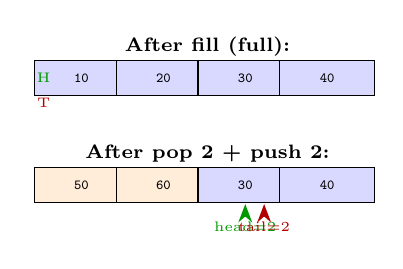
\begin{tikzpicture}[>=Stealth, scale=0.8]
  % State 1: after fill
  \node[font=\scriptsize\bfseries] at (2, 3.5) {After fill (full):};
  \foreach \i/\v in {0/10, 1/20, 2/30, 3/40} {
    \node[draw, minimum width=1.2cm, minimum height=0.45cm,
          fill=blue!15, font=\tiny\ttfamily] at (\i*1.3, 3) {\v};
  }
  \node[font=\tiny, green!60!black] at (-0.6, 3) {H};
  \node[font=\tiny, red!70!black] at (-0.6, 2.6) {T};

  % State 2: after pop 2, push 2
  \node[font=\scriptsize\bfseries] at (2, 1.8) {After pop 2 + push 2:};
  \foreach \i/\v/\c in {0/50/orange!15, 1/60/orange!15, 2/30/blue!15, 3/40/blue!15} {
    \node[draw, minimum width=1.2cm, minimum height=0.45cm,
          fill=\c, font=\tiny\ttfamily] at (\i*1.3, 1.3) {\v};
  }
  \draw[->, thick, green!60!black] (2*1.3, 0.8) -- (2*1.3, 1.0)
    node[below=0.1cm, font=\tiny] {head=2};
  \draw[->, thick, red!70!black] (2*1.3+0.3, 0.8) -- (2*1.3+0.3, 1.0)
    node[below=0.1cm, font=\tiny] {tail=2};
\end{tikzpicture}
\end{center}

\vspace{0.3em}
\begin{block}{Wraparound}
Orange slots were written \emph{after} tail wrapped past index~3
back to index~0. The FIFO order (30, 40, 50, 60) is preserved.
\end{block}
\end{column}
\end{columns}
\end{frame}

% ===========================================================================
\section{Embedded Use Case}
% ===========================================================================

\begin{frame}[fragile]{Use Case: UART Receive Buffer (ISR Producer)}
\begin{columns}[T]
\begin{column}{0.52\textwidth}
\begin{lstlisting}[style=cstyle,
  title={ISR pushes, main loop pops}]
#include "tiku_kits_ds_ringbuf.h"

static struct tiku_kits_ds_ringbuf uart_rx;

void uart_init(void)
{
    tiku_kits_ds_ringbuf_init(&uart_rx, 32);
}

/* Called from UART RX interrupt */
void uart_rx_isr(void)
{
    int32_t byte = (int32_t)UCA0RXBUF;
    /* Push received byte; drop if full */
    tiku_kits_ds_ringbuf_push(
        &uart_rx, byte);
}

/* Called from main loop */
int uart_read(uint8_t *ch)
{
    tiku_kits_ds_elem_t val;
    if (tiku_kits_ds_ringbuf_pop(
            &uart_rx, &val)
        == TIKU_KITS_DS_OK) {
        *ch = (uint8_t)val;
        return 1;
    }
    return 0;  /* no data available */
}
\end{lstlisting}
\end{column}

\begin{column}{0.44\textwidth}
\begin{center}
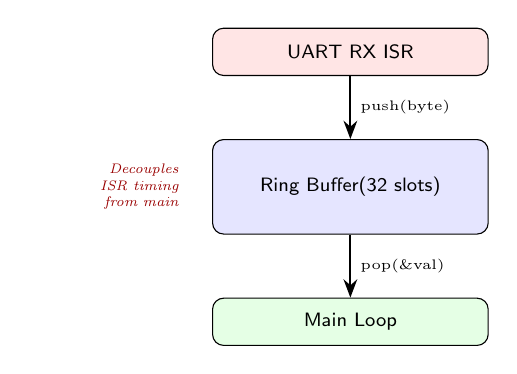
\begin{tikzpicture}[>=Stealth, node distance=0.5cm]
  \node[draw, rounded corners, fill=red!10,
        minimum width=3.5cm, minimum height=0.6cm,
        font=\scriptsize\sffamily] (isr) {UART RX ISR};
  \node[draw, rounded corners, fill=blue!10,
        minimum width=3.5cm, minimum height=1.2cm,
        font=\scriptsize\sffamily, below=0.8cm of isr] (buf)
    {Ring Buffer\\(32 slots)};
  \node[draw, rounded corners, fill=green!10,
        minimum width=3.5cm, minimum height=0.6cm,
        font=\scriptsize\sffamily, below=0.8cm of buf] (main)
    {Main Loop};

  \draw[->, thick] (isr) -- node[right, font=\tiny] {push(byte)} (buf);
  \draw[->, thick] (buf) -- node[right, font=\tiny] {pop(\&val)} (main);

  \node[left=0.3cm of buf, font=\tiny\itshape, text=red!60!black,
        text width=1.8cm, align=right] {Decouples\\ISR timing\\from main};
\end{tikzpicture}
\end{center}

\vspace{0.5em}
\begin{block}{ISR / Main-Loop Pattern}
\begin{itemize}
  \item ISR runs at interrupt priority --- must be fast
  \item Ring buffer absorbs bursts
  \item Main loop drains at its own pace
  \item No dynamic allocation in ISR context
\end{itemize}
\end{block}

\begin{alertblock}{Single Producer, Single Consumer}
This pattern is safe without locks when there is exactly one
producer (ISR) and one consumer (main loop) and the
\texttt{count} field is accessed atomically (16-bit on MSP430).
\end{alertblock}
\end{column}
\end{columns}
\end{frame}

% ---------------------------------------------------------------------------
\begin{frame}[fragile]{Use Case: Last-N Sensor Samples}
\begin{lstlisting}[style=cstyle,
  title={Keep last N readings for processing}]
#include "tiku_kits_ds_ringbuf.h"

#define HISTORY_SIZE 8
static struct tiku_kits_ds_ringbuf history;

void history_init(void) {
    tiku_kits_ds_ringbuf_init(&history, HISTORY_SIZE);
}

void history_add(int32_t reading) {
    if (tiku_kits_ds_ringbuf_full(&history)) {
        tiku_kits_ds_elem_t discard;
        tiku_kits_ds_ringbuf_pop(&history, &discard);  /* drop oldest */
    }
    tiku_kits_ds_ringbuf_push(&history, reading);
}

int32_t history_newest(void) {
    /* Peek returns the head (oldest). To get newest we would need
     * to track it separately, or pop all and re-push. For simple
     * "latest" tracking, the array module may be more convenient. */
    tiku_kits_ds_elem_t val;
    tiku_kits_ds_ringbuf_peek(&history, &val);
    return val;  /* returns oldest */
}
\end{lstlisting}
\end{frame}

% ===========================================================================
\section{Memory Layout}
% ===========================================================================

\begin{frame}{Memory Layout and Sizing}
\begin{columns}[T]
\begin{column}{0.48\textwidth}
\begin{center}
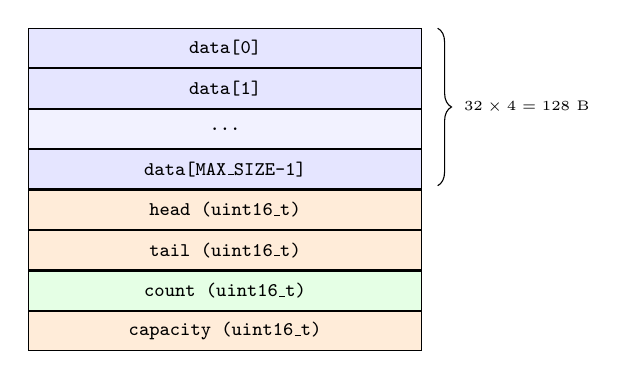
\begin{tikzpicture}[>=Stealth, node distance=0.0cm]
  \node[draw, minimum width=5cm, minimum height=0.5cm,
        fill=blue!10, font=\scriptsize\ttfamily] (d0) {data[0]};
  \node[draw, minimum width=5cm, minimum height=0.5cm,
        fill=blue!10, font=\scriptsize\ttfamily, below=0cm of d0] (d1) {data[1]};
  \node[draw, minimum width=5cm, minimum height=0.5cm,
        fill=blue!5, font=\scriptsize\ttfamily, below=0cm of d1] (d2) {...};
  \node[draw, minimum width=5cm, minimum height=0.5cm,
        fill=blue!10, font=\scriptsize\ttfamily, below=0cm of d2] (dn) {data[MAX\_SIZE-1]};
  \node[draw, minimum width=5cm, minimum height=0.5cm,
        fill=orange!15, font=\scriptsize\ttfamily, below=0cm of dn] (hd) {head (uint16\_t)};
  \node[draw, minimum width=5cm, minimum height=0.5cm,
        fill=orange!15, font=\scriptsize\ttfamily, below=0cm of hd] (tl) {tail (uint16\_t)};
  \node[draw, minimum width=5cm, minimum height=0.5cm,
        fill=green!10, font=\scriptsize\ttfamily, below=0cm of tl] (ct) {count (uint16\_t)};
  \node[draw, minimum width=5cm, minimum height=0.5cm,
        fill=orange!15, font=\scriptsize\ttfamily, below=0cm of ct] (cp) {capacity (uint16\_t)};

  \draw[decorate, decoration={brace, amplitude=5pt}]
    (2.7, 0.25) -- (2.7, -1.75)
    node[midway, right=6pt, font=\tiny] {$32 \times 4 = 128$ B};
\end{tikzpicture}
\end{center}
\end{column}

\begin{column}{0.48\textwidth}
\begin{block}{Size Formula}
\[
  \text{Total} = \texttt{MAX\_SIZE} \times \texttt{sizeof(elem\_t)} + 8
\]
\end{block}

\begin{table}
\centering
\scriptsize
\begin{tabular}{@{}rrr@{}}
\toprule
\textbf{MAX\_SIZE} & \textbf{elem\_t} & \textbf{Total (bytes)} \\
\midrule
8   & int32\_t & 40 \\
16  & int32\_t & 72 \\
32  & int32\_t & 136 \\
32  & int16\_t & 72 \\
\bottomrule
\end{tabular}
\end{table}

\vspace{0.3em}
\begin{alertblock}{Count Field Advantage}
A separate \texttt{count} field means all \texttt{capacity}
slots are usable. Classic head/tail-only designs waste one
slot to distinguish full from empty.
\end{alertblock}
\end{column}
\end{columns}
\end{frame}

% ===========================================================================
\section{Complexity}
% ===========================================================================

\begin{frame}{Time Complexity}
\begin{table}
\centering
\begin{tabular}{@{}lcc@{}}
\toprule
\textbf{Operation} & \textbf{Best Case} & \textbf{Worst Case} \\
\midrule
\texttt{init}   & $O(n)$ & $O(n)$ \\
\texttt{push}   & $O(1)$ & $O(1)$ \\
\texttt{pop}    & $O(1)$ & $O(1)$ \\
\texttt{peek}   & $O(1)$ & $O(1)$ \\
\texttt{clear}  & $O(1)$ & $O(1)$ \\
\texttt{count}  & $O(1)$ & $O(1)$ \\
\texttt{full}   & $O(1)$ & $O(1)$ \\
\texttt{empty}  & $O(1)$ & $O(1)$ \\
\bottomrule
\end{tabular}
\end{table}

\vspace{0.5em}
\begin{block}{All Core Operations Are $O(1)$}
\begin{itemize}
  \item No element shifting --- modulo arithmetic replaces data movement
  \item \texttt{init} is $O(n)$ due to \texttt{memset} zeroing the data array
  \item Deterministic timing makes the ring buffer ideal for ISR contexts
  \item Total cycle count per push/pop is constant regardless of occupancy
\end{itemize}
\end{block}
\end{frame}

% ===========================================================================
\section{Test Suite}
% ===========================================================================

\begin{frame}{Test Cases Overview}
\begin{table}
\centering
\small
\begin{tabular}{@{}clp{7cm}@{}}
\toprule
\textbf{\#} & \textbf{Test Function} & \textbf{What It Verifies} \\
\midrule
1 & \texttt{test\_kits\_ds\_ringbuf\_init}
  & Initialization, capacity bounds, empty/full state \\
2 & \texttt{test\_kits\_ds\_ringbuf\_push\_pop}
  & Push/pop FIFO order, empty-pop error \\
3 & \texttt{test\_kits\_ds\_ringbuf\_wraparound}
  & Tail and head wrap correctly, FIFO preserved \\
4 & \texttt{test\_kits\_ds\_ringbuf\_peek}
  & Peek returns head, does not remove, updates after pop \\
5 & \texttt{test\_kits\_ds\_ringbuf\_full\_empty}
  & Full/empty flags, push-when-full error \\
6 & \texttt{test\_kits\_ds\_ringbuf\_overwrite\_check}
  & Push on full returns error, no silent overwrite \\
7 & \texttt{test\_kits\_ds\_ringbuf\_count\_tracking}
  & Count increments/decrements, mixed ops with wrap \\
8 & \texttt{test\_kits\_ds\_ringbuf\_clear\_reset}
  & Clear resets state, pop after clear fails, re-init works \\
9 & \texttt{test\_kits\_ds\_ringbuf\_null\_inputs}
  & All functions reject NULL with ERR\_NULL \\
\bottomrule
\end{tabular}
\end{table}
\end{frame}

% ===========================================================================
\section{Summary}
% ===========================================================================

\begin{frame}{Summary}
\begin{columns}[T]
\begin{column}{0.48\textwidth}
\begin{block}{What We Built}
\begin{itemize}
  \item Fixed-size circular (ring) buffer
  \item 8 API functions: init, push, pop, peek, clear, count, full, empty
  \item $O(1)$ push and pop via modulo wrap
  \item Count field --- no wasted slot
  \item Zero heap usage --- fully static
\end{itemize}
\end{block}

\begin{block}{Key Design Choices}
\begin{itemize}
  \item Separate \texttt{count} field distinguishes full/empty
  \item No silent overwrite on full --- caller decides policy
  \item Modulo arithmetic avoids branching
  \item NULL-pointer validation on all functions
\end{itemize}
\end{block}
\end{column}

\begin{column}{0.48\textwidth}
\begin{block}{Use Cases}
\begin{itemize}
  \item UART / SPI receive buffers
  \item Last-N sensor sample history
  \item ISR-to-main-loop event queues
  \item Streaming audio or signal pipelines
\end{itemize}
\end{block}

\begin{block}{Files}
\scriptsize
\begin{tabular}{@{}lp{4.5cm}@{}}
Common: & \texttt{ds/tiku\_kits\_ds.h} \\
Header: & \texttt{ds/ringbuf/tiku\_kits\_ds\_ringbuf.h} \\
Source: & \texttt{ds/ringbuf/tiku\_kits\_ds\_ringbuf.c} \\
Tests:  & \texttt{tests/ds/test\_kits\_ds\_ringbuf.c} \\
\end{tabular}
\end{block}
\end{column}
\end{columns}
\end{frame}

% ---------------------------------------------------------------------------
\begin{frame}{Thank You}
\begin{center}
\Large\textbf{TikuKits DS: Ring Buffer}\\[0.5em]
\normalsize Constant-Time Circular Buffers for Embedded Systems\\[1.5em]

\begin{tabular}{rl}
  Repository: & \url{https://github.com/tikuos/tikuOS} \\
  License:    & Apache 2.0 \\
  Common:     & \texttt{tikukits/ds/tiku\_kits\_ds.h} \\
  Header:     & \texttt{tikukits/ds/ringbuf/tiku\_kits\_ds\_ringbuf.h} \\
  Source:     & \texttt{tikukits/ds/ringbuf/tiku\_kits\_ds\_ringbuf.c} \\
  Tests:      & \texttt{tikukits/tests/ds/test\_kits\_ds\_ringbuf.c} \\
\end{tabular}
\end{center}
\end{frame}

\end{document}
